\subsection{Training Recipe}
Our training recipe consists of four stages: supervised fine-tuning~(SFT), two-stage RLHF for hybrid thinking, reasoning RL with length control, and agentic RL with action-centric rubrics.

\subsubsection{SFT}
\begin{figure*}[t!]
    \centering
    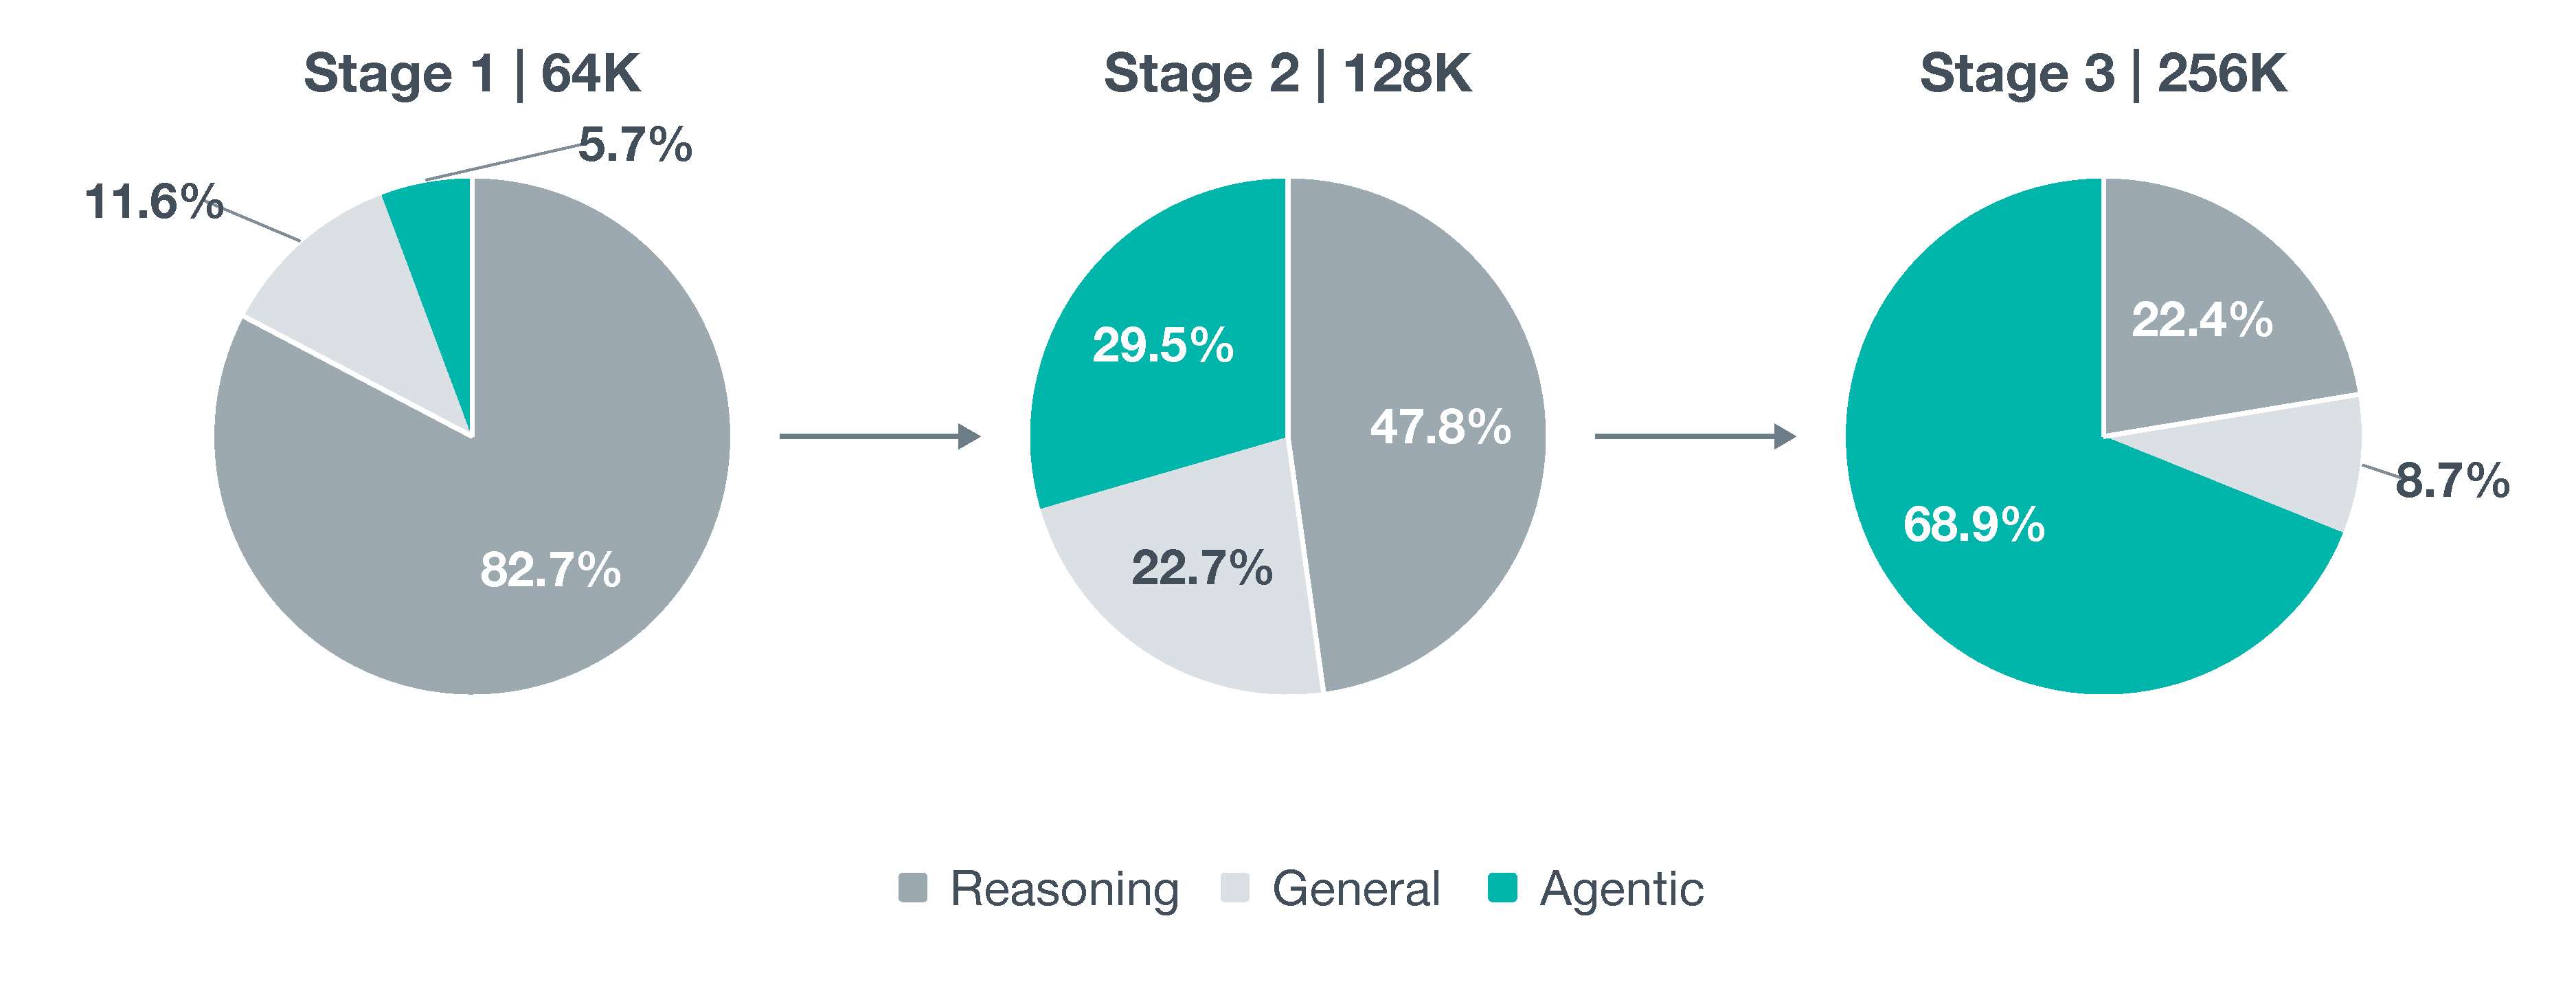
\includegraphics[width=0.8\textwidth]{sft_stage_mix.pdf}
    \caption{Stage-wise SFT target-token mixtures for the 64K, 128K, and 256K stages.}
    \label{fig:sft-stage-mixture}
\end{figure*}

Starting from the pretrained checkpoint, we conduct supervised fine-tuning with a three-stage curriculum that progressively extends the maximum training context from 64K to 128K and 256K tokens. Rather than maintaining a fixed data mixture, we gradually shift the distribution of supervised target tokens from STEM-centered reasoning toward long-horizon agentic interaction as the model develops a stronger reasoning foundation.

\paratitle{Three-Stage Curriculum.}
In the 64K stage, the supervised target-token mixture is dominated by reasoning-oriented STEM data (82.7\%), with 11.6\% general instruction data and 5.7\% agentic data. This stage establishes the foundation for scientific, mathematical, and engineering problem solving. In the 128K stage, the mixture shifts to 47.8\% reasoning-oriented STEM data, 22.7\% general instruction data, and 29.5\% agentic data, providing a transition toward longer-context instruction following, tool use, and multi-turn environment interaction.
After the model acquires a sufficiently strong reasoning foundation, the 256K stage shifts the primary training objective toward agentic capability. We allocate 68.9\% of the supervised target tokens to agentic data, while retaining 22.4\% reasoning-oriented STEM data and 8.7\% general instruction data. This strengthens long-horizon planning, tool invocation, execution feedback utilization, and recovery from intermediate failures. The three-stage mixtures are summarized in Figure~\ref{fig:sft-stage-mixture}.




\paratitle{Turn-Level Loss Masking.}
A successful trajectory may still contain incorrect or unproductive intermediate turns. We assign a binary loss mask $m_t$ to each assistant turn using execution feedback and rubric-based assessment. Unreliable turns are excluded from the SFT loss ($m_t=0$) but retained, together with their resulting observations, in the context of subsequent turns. This preserves the full interaction context without training on incorrect turns, allowing the model to learn how to recover from mistakes in long-horizon tasks.


% \subsubsection{RL}
\subsubsection{Two-Stage RLHF for Hybrid Thinking}

After mixed-domain SFT, the compact model still exhibits unstable generation behaviors, including repetitive reasoning, cyclic reflection, delayed termination, duplicated answers, malformed formats, and abnormal continuations. To address these failure cases and establish a stable foundation for subsequent reasoning and agentic RL, we first apply a two-stage RLHF procedure covering both think and non-think responses. 

We train a point-wise reward model that independently evaluates the overall
quality of each response. 
The reward favors responses that are correct, relevant, well formatted, and
properly terminated, while discouraging repetition, ineffective continuation,
and malformed outputs. In addition, the reward takes both safety and user-friendliness into account to ensure that the model maintains harmless and friendly interactions while adhering to the specified generation behavior.
A central finding is that the behavioral regularization learned
from general-purpose RLHF exhibits strong generalization along two distinct
dimensions:

\textbf{Cross-task generalization.}
General-purpose RLHF improves not only instruction following but also
mathematical reasoning, coding, and agentic performance. This observation
challenges the conventional view of RLHF as primarily a mechanism for
controlling safety and conversational style. Instead, behaviors such as
avoiding repetition, respecting output formats, and terminating appropriately
act as a form of trajectory-level regularization. In complex agent tasks, many
failures are caused not by incorrect reasoning, but by generation loops,
malformed outputs, or abnormal continuations that interrupt downstream
execution. Removing these failures allows the model's existing reasoning
capabilities to be expressed more reliably.

\textbf{Cross-mode generalization.}
Behavioral constraints learned predominantly from Non-Think responses generalize
directly to Think-mode generation. Although the second stage mainly trains on non-think responses to general queries, it also markedly
reduces cyclic reflection, redundant reasoning, and abnormal continuation in
Think mode. This indicates that structured generation, repetition control, and
termination awareness are not mode-specific skills, but shared capabilities
underlying both response modes. 

To provide a concise illustration of these improvements,
Table~\ref{tab:rlhf-main-results} reports representative results across three
capability categories: AA-LCR\footnote{https://huggingface.co/datasets/ArtificialAnalysis/AA-LCR} for alignment, LiveCodeBench-V6~\cite{jain2024livecodebenchholisticcontaminationfree} for reasoning,
and PinchBench-V2\footnote{https://pinchbench.com/} for agentic capability. For each benchmark, we compare accuracy,
average output length, and bad-case rate (percentage of data with formatting errors or exceeding the length limit) across the SFT, Think-RLHF, and final
Think-to-Non-Think RLHF checkpoints. All checkpoints are evaluated in Think
mode under the same decoding configuration. These three benchmarks
 consistently show that the two-stage RLHF procedure improves task performance while producing
shorter and more stable generation trajectories.


\begin{table*}[t]
    \centering
    \small
    \setlength{\tabcolsep}{4pt}
    \renewcommand{\arraystretch}{1.10}

    \begin{tabular}{@{}llrrr@{}}
        \toprule
        \multirow[c]{2}{*}{\textbf{Capability}}  & \multirow[c]{2}{*}{\textbf{Metric}}   & \multicolumn{3}{c}{\textbf{Training Stage}} \\
        \cmidrule(lr){3-5}  
        & & \textbf{SFT}  & \textbf{Think RLHF}  & \textbf{Non-Think RLHF} \\
        \midrule

        \multirow{3}{*}{\makecell[l]{Alignment\\\textit{AA-LCR}}}
        & Accuracy (\%) $\uparrow$
        & 50.00 & 53.00 & \bfseries 57.00 \\
        & Bad-case Rate (\%) $\downarrow$
        & 17.00 & 8.00 & \bfseries 2.00 \\
        & Average Length (tokens) $\downarrow$
        & 19,545 & 13,791 & \bfseries 7,915 \\
        \midrule
        
        \multirow{3}{*}{\makecell[l]{Reasoning\\\textit{LiveCodeBench-V6}}}
        & Accuracy (\%) $\uparrow$
        & 65.45 & 68.51 & \bfseries 72.10 \\
        & Bad-case Rate (\%) $\downarrow$
        & 6.49 & 0.95 & \bfseries 0.00 \\
        & Average Length (tokens) $\downarrow$
        & 25,905 & 16,781 & \bfseries 15,182 \\
        \midrule
        
        \multirow{3}{*}{\makecell[l]{Agentic\\\textit{PinchBench-V2}}}
        & Accuracy (\%) $\uparrow$
        & 55.89 & 71.14 & \bfseries 75.49 \\
        & Bad-case Rate (\%) $\downarrow$
        & 5.44 & 8.16 & \bfseries 2.72 \\
        & Average Length (tokens) $\downarrow$
        & 20,515 & 13,098 & \bfseries 11,808 \\
        
        \bottomrule
    \end{tabular}

    \caption{
    Representative effects of two-stage RLHF on alignment, reasoning, and
    agentic capabilities. All checkpoints are evaluated in Think mode under
    identical decoding settings.
    }
    \label{tab:rlhf-main-results}
\end{table*}



\subsubsection{Reasoning RL with Length Control}

 Following general-purpose RLHF, we further conduct reasoning RL to strengthen Think-mode capability. Unlike Nanbeige4.1, where reasoning RL optimized primarily for task performance, this version pursues accuracy gains while simultaneously constraining reasoning length. To this end, we introduce a problem-dependent length-control objective for Think-mode RL. The objective combines a fixed length budget with a continuous, difficulty-aware penalty, encouraging concise reasoning on reliably solved problems while preserving exploration on difficult ones.

\textbf{Offline budget construction.}
For each problem $q$, we collect successful historical rollouts from checkpoints preceding this stage and set its length budget $b_q$ to the median length of these correct responses. The budgets are computed once and remain fixed throughout the training process.

\textbf{Difficulty-aware length penalty.}
Training alternates between a \emph{constrained} phase, which penalizes
over-long responses, and a \emph{free-expansion} phase, which disables the
penalty to preserve exploration. The steps in each phase are two
separate hyperparameters. In constrained phase, given a response of
length $L_i$, maximum rollout length $L_{\max}$, and base task reward
$r_i^{\mathrm{base}}$, we shape the final reward as:
\begin{equation}
r_i = r_i^{\mathrm{base}} - \alpha\, p_q
\left[\frac{L_i-b_q}{L_{\max}-b_q}\right]_0^1,
\end{equation}
where $[x]_0^1=\min(\max(x,0),1)$, $\alpha>0$ bounds the penalty magnitude, and
$p_q$ is the fraction of fully correct responses in the current rollout group.
The penalty is thus difficulty-aware: responses within budget are never
penalized, while the penalty for over-budget responses grows with both the normalized excess length and the problem's current pass rate, so concise reasoning is encouraged on reliably solved problems but not on still-difficult ones.
Because the penalty is subtracted rather than gating the task reward, it
preserves correctness differences and remains continuous at the budget
boundary; for binary rewards, $\alpha<1$ further guarantees that a correct
response is always preferred to an incorrect one regardless of length.
\begin{comment}
    

\end{comment}

% \paratitle{Action-Centric Rubrics for Process-Rewarded Agent Training}
\subsubsection{Agentic RL with Action-Centric Rubrics.}

Across diverse agentic settings, including general-purpose tool use, search, cowork, and coding, we design action-evaluation rubrics to diagnose and assess behavioral deficiencies in agents. These rubrics measure dimensions such as tool-call accuracy and the information gain each turn contributes toward task completion, and their scores serve as process-level rewards that penalize recurrent action errors at the turn level.

Data selection is equally important at this scale. Using the reasoning-RL model to estimate task pass rates, we restrict agentic RL to relatively easy tasks, namely those with short trajectories and relative higher pass@8 score. For a compact model, we find that such tasks yield both more stable optimization and larger performance gains than harder or longer-horizon ones.

\begin{figure}
    \centering
    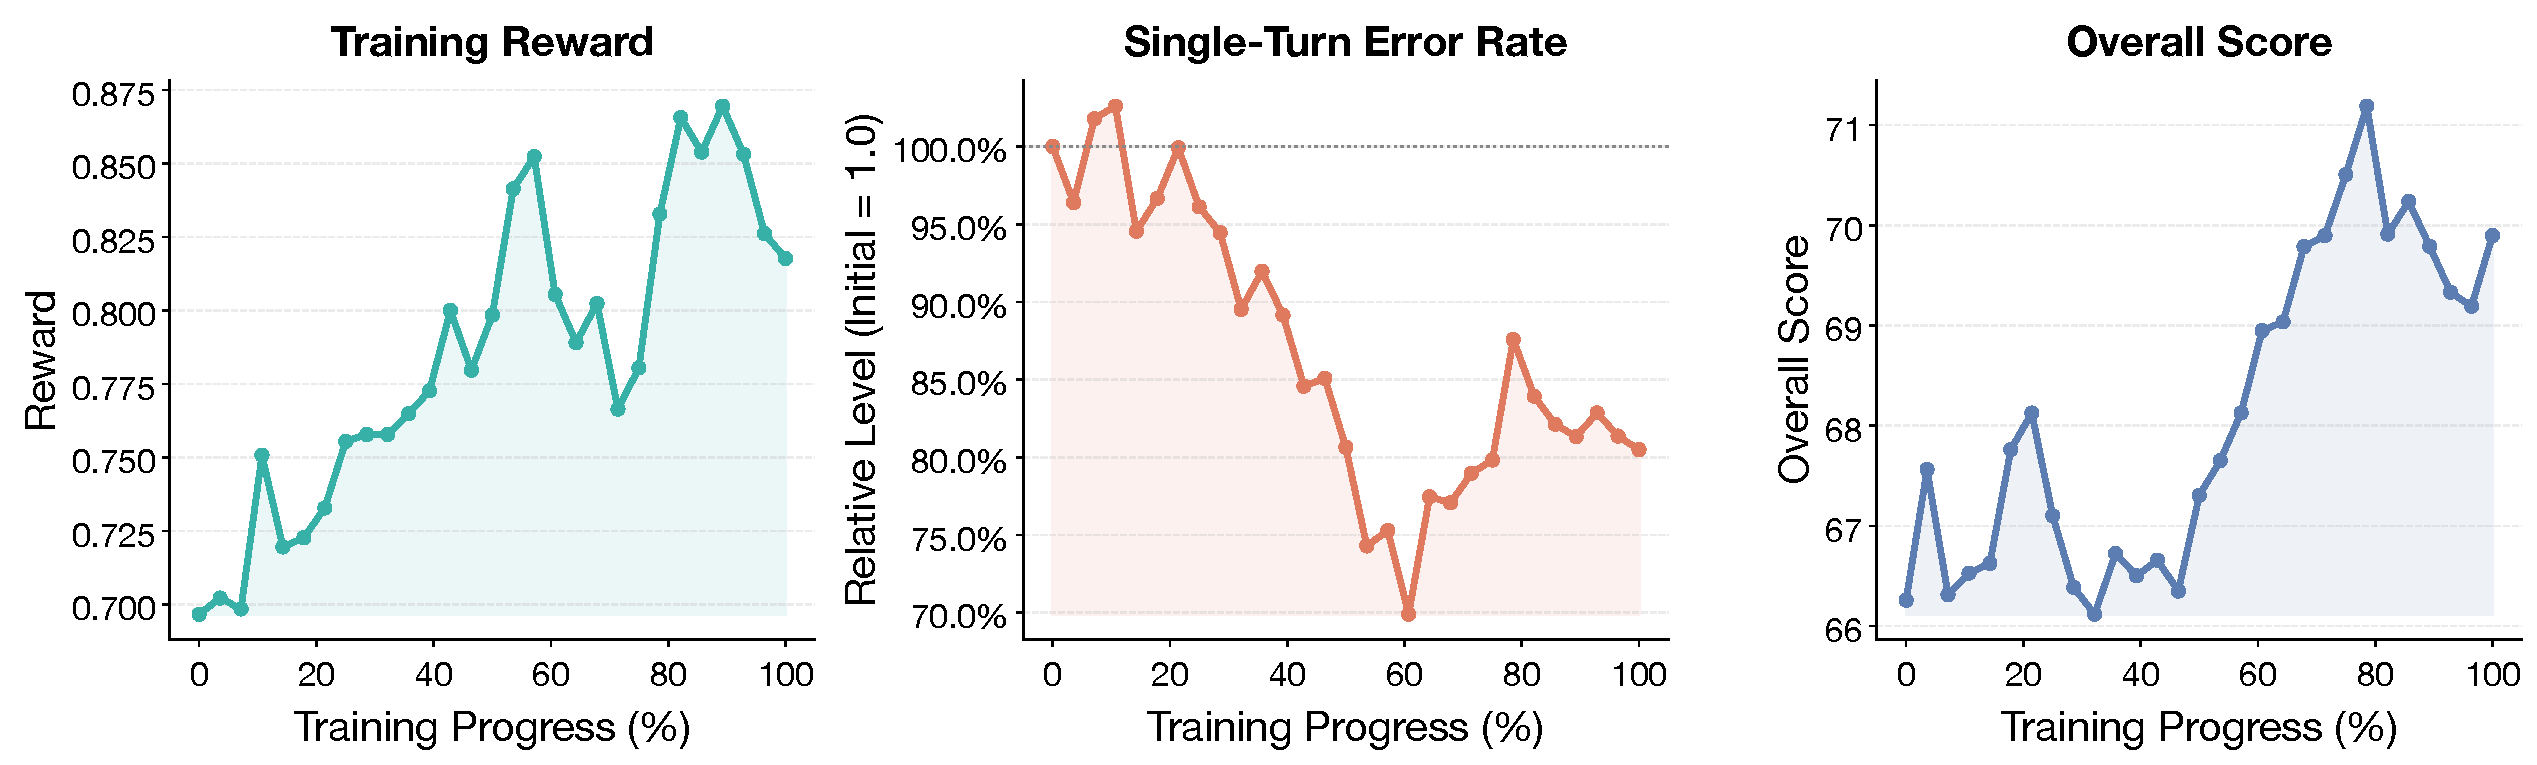
\includegraphics[width=1\linewidth]{figures/training_dynamics.pdf}
    \caption{Training Dynamics with Action-Centric Agentic RL.}
    \label{fig:training_dynamics}
\end{figure}


With this data and reward design, we run agentic RL and track its dynamics on the Rapid Validation Tasks mentioned in Sec~\ref{sec:rapid_validation}. We report the single-turn action error rate, normalized by the initial checkpoint, together with the overall task score, as shown in Figure~\ref{fig:training_dynamics}. Despite fluctuations caused by the diversity of trajectories and task difficulty, the training reward exhibits an overall upward trend. Meanwhile, the normalized action error rate decreases by approximately 20\%, while the overall score improves from 66.0 to a peak of 71.0 during training. These results show that combining outcome and action-centric process rewards suppresses recurrent action errors and improves end-task performance.

\subsubsection{Performance Gains from Reinforcement Learning}

\begin{figure}
    \centering
    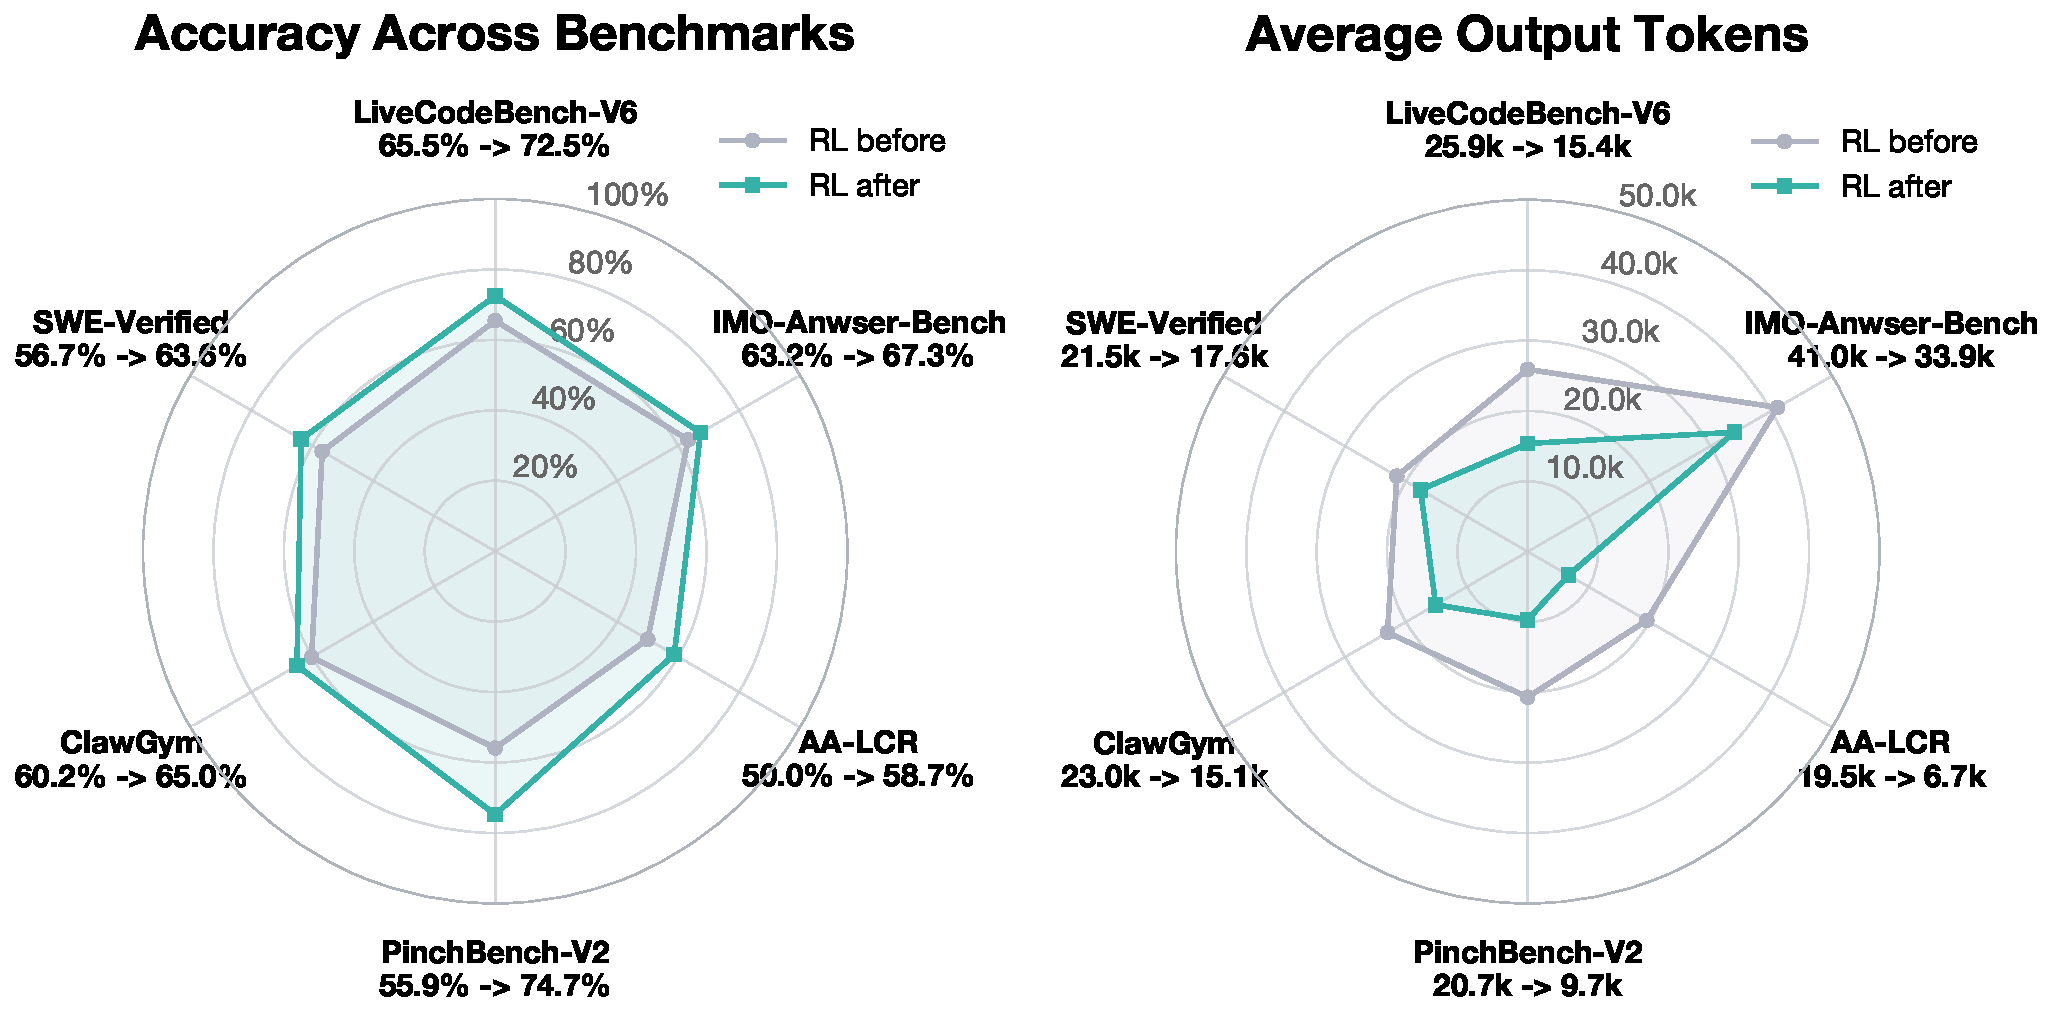
\includegraphics[width=0.9\linewidth]{figures/accuracy_token_radar_side_by_side.pdf}
    \caption{Accuracy and average token usage before and after RL across diverse benchmarks.}
    \label{fig:rl_acc_token_radar}
\end{figure}

To characterize the cumulative effect of the complete RL pipeline, we evaluate
the pre-RL and post-RL checkpoints on six benchmarks covering
mathematical and code reasoning, alignment, software engineering, and agentic
task execution.
As illustrated in Figure~\ref{fig:rl_acc_token_radar}, among these benchmarks, the post-RL checkpoint achieves higher accuracy while using fewer output tokens.